\chapter{\acl{sota}}
\label{chapter:sota}

\section{Datasets}
\label{section:sota:datasets}

Training an autonomous vehicle to be capable of driving himself is a complex challenge with multiple parts and problems to be solve: recognizing other users of the road (persons, vehicles, cyclists); understanding traffic signs; track and estimate the movement of the road users; plan the path; accurate modelling of the environment; among many others. To both train neural networks and other genetic algorithms, but also to intensively test systems and other software, huge amounts of data are required.

To accelerate this progress, a collaborative effort is being made to release datasets online for free public usage under permissive licenses. This datasets vary in their objective, sensory data available, conditions whose data has been acquired, driving conditions and format on which they are provided, among other aspects. 

Despite this work having no intentions to study autonomous driving, the algorithms developed for calibration, sensor fusion and computing the correspondence between objects of interest in image and point cloud are not meant to be particular applied on datasets with interference. Therefore, using public available datasets not only allow the development of those algorithms before experimental data can be gathered, but also widen the applicability of such work, without losing their applicability to the particular situation of \ac{lidar} interference.

During the months when this research work was carried, several new datasets were made available online, such as nuScenes~\cite{nuScenes2019} and Waymo~\cite{Waymo}. Since no new contribute was expected from their usage besides the ones already provided by the datasets already in use on this research, no further research on them was carried. 

For the purposes of this research, several datasets were considered and tested. On the next sections, a brief summary is given about the ones that have sensory data from camera and \ac{lidar}. Those were the candidates to be used on this work.

\subsection{Ford Campus \acl{lidar} dataset}
Gathered in 2009, in Michigan, the Ford Campus \ac{lidar} dataset contains camera, \ac{lidar}, \ac{imu} and \ac{gps} data. The dataset consists of two test scenarios, one inside the Ford Research campus and another on downtown Dearborn. A small subset of the former test scenario is also provided.

The data is provided in raw format, accompanied by log files with timestamps, \ac{gps} and \ac{lcm}\footnote{For more information on \acf{lcm} protocol for estimating delays between the registered of sensory data on master-slave systems, see~\cite{VelodyneHDL64}.} logs with all raw data. The images from an omnidirectional camera, a Point Grey Ladybug3, are stored on \ac{ppm}; \ac{lidar} data from a Velodyne HDL-64E on \ac{pcap} format, from the \ac{tcp} connection socket; two Riegl LMS-Q120 \acp{lidar} also provide more information on the scan.

The data is rectified and synced under \ac{matlab} \textit{.mat} files. Along with the raw data and synced and rectified \textit{.mat} files, source code is also provided for parsing the raw data, visualizing the \ac{lcm} logs and pre-processed data on \ac{matlab}. A C and \ac{opengl} software that can render textured point clouds is also available.

The modified Ford F-250 pickup truck, which can be seen on figure~\ref{fig:sota:ford_sensors}, uses 3 sensors for navigation~\cite{Pandey2011}: one 3D \ac{lidar}, Velodyne HDL-64E \ac{lidar}~\cite{VelodyneHDL64}; one camera: Point Grey Ladybug3 omnidirectional camera; and two 2D \acp{lidar}: Riegl LMS-Q120 lidar. More details about the sensors, their relative positioning and data formats and files can be found~\cite{Pandey2011}.

\begin{figure}
	\centering
	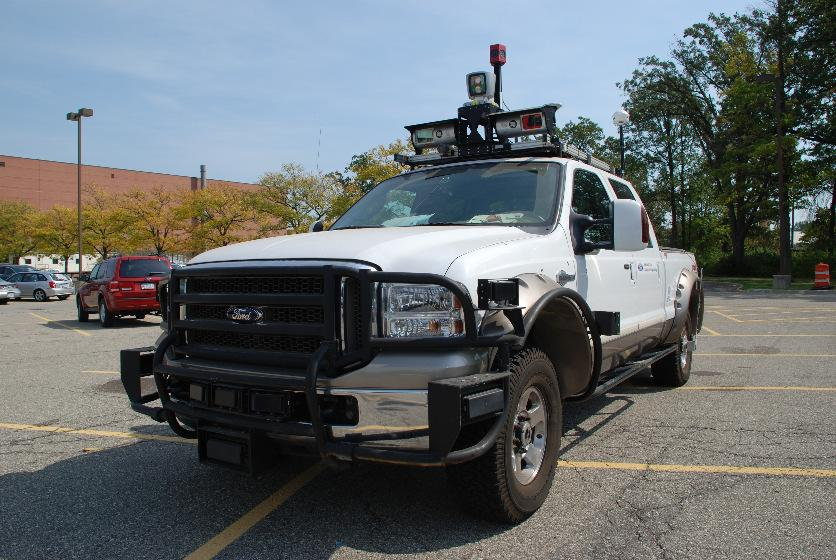
\includegraphics[width=0.5\textwidth]{img/sensor_fusion/ford_sensors.jpg}
	\caption{Ford 250 pickup equipped with the sensors described in the previous paragraphs. On the top, the Ladybug omnidirectional camera, on the back the \ac{imu} and \ac{gps} unit. }
	\label{fig:sota:ford_sensors}
\end{figure}


\subsection{\acl{kitti} Dataset}
A well known dataset for researchers of computer vision, autonomous driving and \ac{ml}, \ac{kitti} was recorded in 2011 and released for the public in 2013. This dataset contains various driving scenarios: suburban, highways, residential and campus areas; with trucks, cars, cyclists and persons. Alongside with data for testing, calibration measures are provided for all sensors.

The test car, a Volkswagen Passat is equipped with two stereo pairs, one with color and other with gray cameras, a \ac{lidar}, an \ac{imu} and a\ac{gps} sensor. Data from all four cameras is stored on \ac{png} format, \ac{lidar} measurements as a binary float matrix, \ac{gps} and {imu} data textually. Additionally to the raw data, logs containing the timestamps and the transforms between the sensors are also provided. Labeled data is also available for some test scenarios on \ac{xml} files.

Along with the data and calibration parameters, several tools written in C++ or \ac{matlab} are also provided. The dataset offers two types of data categories: (1) unsynced and unrectified data or (2) synced and rectified data. 

The sensory apparatus contains 2 PointGray Flea2 greyscale and color cameras, a Velodyne HDL-64E \ac{lidar}~\cite{VelodyneHDL64}, among others less relevant sensors~\cite{Geiger2013a}.

\begin{figure}
	\centering
	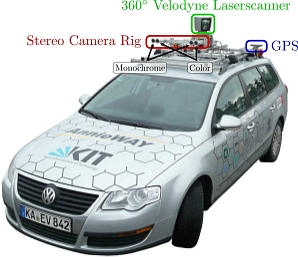
\includegraphics[width=0.5\textwidth]{img/sensor_fusion/passat_sensors.jpg}
	\caption{Volkswagen Passat equipped with the sensors described in the previous paragraphs, for the \ac{kitti} dataset. On the top, the Velodyne \ac{lidar} and below the 2 stereo pairs (color and grey). On the back, the \ac{imu} and {gps} systems are present.}
	\label{fig:sota:kitti_sensors}
\end{figure}


\subsection{Udacity Self-Driving Car Nanodegree Dataset}
Available publicly is also the data from Udacity online course on self-driving car. This dataset dates back to 2016 and was gathered with the intent to develop a level 4 autonomy vehicle, containing much more data diversity than the previous two. The data available contains images from 3 color cameras, a \ac{lidar} data, \ac{imu} and \ac{gps}, among other sensory data, such as speed, braking, etc.

Their data is not available in raw format, only structured in \ac{ros} \textit{.bag} files. Some tools for visualizing and interacting with their data are provided for \ac{ros}~\cite{udacity}. 

Not much information is publicly available, and the dataset contains to calibration data between its sensors.

\subsection{Summary}
Table~\ref{tab:sota:datasets_comparison} summarizes all the relevant data from the datasets~\cite{udacity, Pandey2011, Geiger2013a}. One notices that while there are few differences between the relevant types of data gather, major differences can be observed on the format in which they are provided. 

The diversity of scenarios and size of the dataset is also an aspect to considered. On this matter, \ac{kitti} and Udacity's are superior to Ford dataset, with \ac{kitti} providing the largest dataset in quantity, with already rectified and synced data. 

While Udacity dataset is the newest and provides direct out-off-the-shelf integration with \ac{ros}, that type of integration can also be achieved for \ac{kitti} by using other tools, such as \textit{kitti2bag}~\cite{TomasKrejci}. 
	
\begin{table}[H]
	 \rowcolors{4}{gray!10}{white}
	 \renewcommand{\arraystretch}{1.2}
	 \centering
	\begin{tabular}{llccc}
																& & \multicolumn{3}{c}{Datasets} \\ \cline{3-5}
																& & Ford Campus  & \acs{kitti} & Udacity \\ \midrule
																%
																& \ac{lidar}	   & \checkmark  & \checkmark & \checkmark \\ 
																& Color Camera	 & \checkmark  & \checkmark & \checkmark  \\
																& Grey Cameras   &             & \checkmark &  \\
																& Stereo Camera  &             & \checkmark & \checkmark  \\
																& Omnidirectional Camera &  \checkmark  &  &  \\
																& \acs{imu}      & \checkmark  & \checkmark & \checkmark  \\
																& \acs{gps}      & \checkmark  & \checkmark & \checkmark  \\
		\rowcolor{white}\multirow{-8}{*}{Sensors and Data} & Driving data\footnotemark & & & \checkmark \\ \hline
		\multirow{5}{*}{Data Formats and Tools} & Raw data available & \checkmark & \checkmark &  \\
																			 & Data parsing tools & \checkmark & \checkmark & \checkmark  \\
																			 & Rectified data & \checkmark & \checkmark & \checkmark \\
																			 & Synced data & \checkmark & \checkmark &  \checkmark  \\ 
																			 & Calibration parameters & \checkmark  & \checkmark  & \checkmark  \\\hline 
		\multicolumn{2}{l}{Raw data for sensors calibration} & \checkmark & \checkmark & \\
		\multicolumn{2}{l}{Direct \ac{ros} data compatibility} &  & \checkmark & \checkmark \\
		\multicolumn{2}{l}{Data of acquisition} & 2009  & 2011 & 2016 \\
		\bottomrule
	\end{tabular}
\caption{Comparison between the datasets more appropriated to this thesis objectives}
\label{tab:sota:datasets_comparison}
\end{table}
\footnotetext{Other driving data includes, but it is not limited to: vehicle speed, joints states, twist, brakes, suspension, fuel level, \ac{can} bus data, steering, tire pressure, among many others.}

Comparing the 3 datasets, not only using table~\ref{tab:sota:datasets_comparison} but also the previous sections, Udacity and \ac{kitti} are more suited to the purposes of this work. They provide a larger dataset than Ford, have \ac{ros} compatibility and the tools provided are open-source and not developed to be used on proprietary software.

Since Udacity dataset integrates more easily with \ac{ros} than \ac{kitti}, providing also some tools for \ac{ros} preliminary tests, learning and earlier development stages will occur with this dataset. Later, due to the lack of calibration parameters and raw data for sensors calibration\footnote{Note that, despite Udacity dataset not providing data to ease the calibration of its sensors, such as camera intrinsic calibration or the extrinsic calibration between \ac{lidar} and camera, such calibration parameters can be obtained from this data. Those parameters are not accurate as those obtained using a proper calibration setup and are out the scope of this research (being another research topic on itself) and therefore no effort will be dedicated to this topic.}, this research will use the \ac{kitti} dataset.

\section{Camera on computer vision}
Vision is the human sense most relevant to how we perceive the world and how we navigate it~\cite{Ekstrom2015}. Replicating this ability on machines, through the usage of cameras, is a widely researched topic on computer vision and instrumentation~\citeneeded. The most common cameras, as our eyes, take advantage of the pinhole effect: a small hole (or pin), that is used to spatially filter the non-focused light beams through an aperture~\cite{camera_models, Sturm2010}, producing a mirrored, but focused image.

Therefore, to proper use a camera on the field of computer vision, some notions of photography are required. Since this research is focused on the usage of industrial cameras and not consumer cameras, such notions will be simplified to the minimum necessary. 

\subsection{Camera Focus and \acl{dof}}
Focusing a camera can only be attained for an exact distance from the camera~\cite{Merklinger1993, Photopillers}, measured perpendicularly to the plane of focus, which is the plane containing the \ac{cmos} or \ac{ccd} chip. Therefore, on every image, there is a plane of focus and what actually ``looks focused'' is really just ``acceptably sharp focus'', since precise focus is only possible to an exact distance, and not for an entire tridimensional object.

``Acceptably sharp focus'' means that a point in the real world would not result in a point on the image (as happens in precise focus), but in a blurred spot that is circular (due to the form of the aperture)\cite{Photopillers}. However, if the size of blur is small enough, little to no differences can be perceived and the image is considered to be focused\cite{Photopillers}. The maximum size at which this blur is not noticed by the viewer (given a specific sensor size, dimension of the viewed photo, viewing distance and acuity of the viewer) is called the \ac{coc}\cite{Photopillers, Merklinger1993}.

The first step in focusing an image requires the calculation of the hyperfocal distance, $H$: the distance at which the camera is focused to ensure objects from half of this distance to the infinity are in an ``acceptably sharp focus'' (refer to as just focus, from now on). This distance can be calculated using the equation~\ref{eq:hyperfocal_distance}, below, where $f$ is the focal length, $N$ is the F-number and $c$ the \ac{coc} limit. Hyperfocal near limit is defined as $H_{near} = \frac{H}{2}$.

\begin{equation}
	\label{eq:hyperfocal_distance}
	H = \frac{f^2}{Nc} + f \approx \frac{f^2}{Nc} 
\end{equation}

Known the hyperfocal distance, the \acf{dof} can be calculated. \ac{dof} is measured in meters and is the subtraction of the farthest and nearest distance at each objects are focused (see equation~\ref{eq:dof}), indicating the distance between this two points\cite{Photopillers, Merklinger1993, mvg_book}. The nearest and farthest points can be calculated using the equations~\ref{eq:dof_near} and~\ref{eq:dof_far}, respectively.

\begin{subequations}
	\label{eq:dof_all}
	\begin{align}
		DoF & = DoF_{far} - DoF_{near} \label{eq:dof} \\
		DoF_{far} & = \frac{H\times d}{H - (d - f)} \label{eq:dof_far} \\
		DoF_{near} & = \frac{H\times d}{H + (d - f))} \label{eq:dof_near} 
	\end{align}
\end{subequations}

Using equations~\ref{eq:dof_all} is possible to select a desired \acl{dof} for an image that guarantees that all the objects of interest are focused. Taking in consideration that smaller apertures (bigger F-numbers) will increase the exposition time\cite{Merklinger1993}, a target distance can be selected with the guarantee that all the objects from the near \ac{dof} point to the far \ac{dof} will be sharp.

\subsection{Camera Geometry}
A world point in a 3-dimensional Euclidean space can be represented by a vector with 3 real coordinates: $(X, Y, Z)$ and an image pixel of a digital image as an element of a 2D matrix with integer coordinates $(u, v)$. From a mathematical standpoint, a camera can be considered as a mapping tool between the world three dimensions objects into a 2D image plan, such as depicted by equation~\ref{eq:camera_transform}. 

\begin{equation}
	\label{eq:camera_transform}
	(X, Y, Z) \xrightarrow[]{\text{transformation}} (u, v)
\end{equation}

Several camera models exist \cite{camera_models, Sturm2010}, such as weak-perspective, fisheye, affine, etc., but on this work only the pinhole camera model will be considered. The pinhole camera model is based on the pinhole effect, represented on figure~\ref{fig:pinhole_effect}, which states that a small hole (or aperture) can be used to spatially filter the light rays by angle of incidence, reducing the overlapping of the light rays coming from different incident angles through the pinhole. 

\begin{figure}[H]
	\centering
	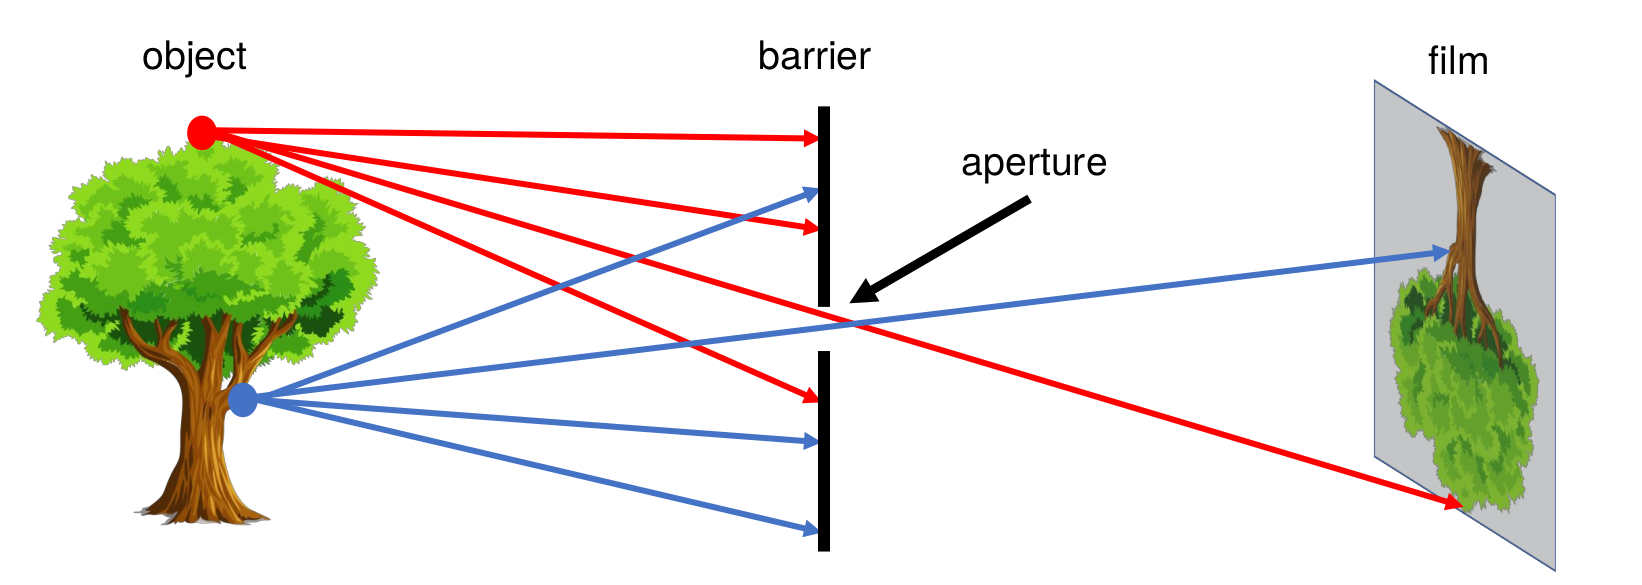
\includegraphics[width=0.6\textwidth]{img/camera/pnhole_effect.png}
	\caption{Pinhole effect on a small aperture. Source: CS231A Course Notes~\cite{camera_models}}
	\label{fig:pinhole_effect}
\end{figure}

The pinhole camera model describes the perspective transformation on equation~\ref{eq:camera_transform} as a central projection where all light rays meet at the camera center, $\mathcal{F}_c$. A diagram of the pinhole camera is shown on figure~\ref{fig:pinhole_camera_model}. On this model, the z axis collinear with the optical axis\footnote{Also called principal axis. The two terms can be used.} , which is the same orientation that the camera is facing. The image plane is at the coordinates $z = f$, where $f$ is the focal length, being intersect by the optical axis on the principal point, with coordinates $(c_x, c_y)$ on the image plane axis. Note that the principal point is not the origin of the coordinates on the image plane, but the middle point, being the origin located on the top left corner, with a downward y axis.

\begin{figure}
\centering
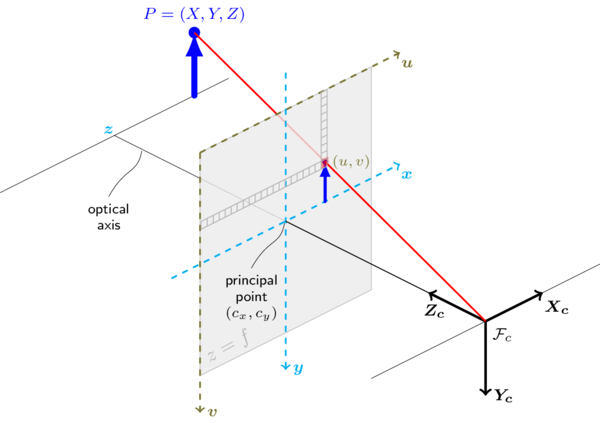
\includegraphics[width=0.6\textwidth]{img/camera/pinhole_camera_model.png}
\caption{Pinhole camera model. Source: \acl{opencv}\cite{opencv_doc}}
\label{fig:pinhole_camera_model}
\end{figure}

When operating with a pinhole camera model, is more convenient to use a Projective Space instead of the more common Euclidean Space\cite{mvg_book}, which has the advantage of all of its points being oriented through a single point, following the visual effect of a central perspective. By using a projective space instead of an Euclidean for addressing the transformations of a pinhole camera model, mathematics become more intuitive and relatable to the actual geometry of the model. Projective spaces use homogeneous coordinates and has non-Euclidean geometry, but that allow for changes between the two\cite{mvg_book, camera_models}.

A tridimensional Euclidean Space can be represented on a Projective space using 3+1 coefficients. Therefore, the previous tridimensional vector can be rewritten in homogeneous coordinates as $(wX, wY, wZ, w)$ \cite{mvg_book}. If $w \neq 0$, we can transform from the Projective to Euclidean Space, obtaining the world representation of such points, by dividing the homogeneous point by $w$. For the cases in which $w =  0$, we have purely projective points at infinity, that only exist in Projective Space~\cite{mvg_book}. 


The relation depicted in equation~\ref{eq:camera_transform} can expressed in projective geometry as:

\begin{equation}
	\begin{bmatrix}
		u \\ v \\ 1
	\end{bmatrix}
= P \times 
\begin{bmatrix}
		X \\ Y \\ Z \\ 1
	\end{bmatrix}, \qquad \text{if } w = 1
\end{equation}

Where $P$ is the projection matrix that performs the transform from world points to image points. The projection matrix in a pinhole camera model is the result of multiplication of two matrices: the camera matrix (or matrix of the camera intrinsic parameters), $K$; and a joint rotation and translation matrix, $[R|t]$, where $R$ is the rotation matrix and $t$ the translation vector. The combination of this matrices is given on equation~\ref{eq:projective_matrix} and the full camera transform is expanded on equation~\ref{eq:camera_transform_full}, through the replacement of equation~\ref{eq:projective_matrix} in~\ref{eq:camera_transform}.

\begin{equation}
	\label{eq:projective_matrix}
	P = K[R|t]
\end{equation}

\begin{equation}
	\label{eq:camera_transform_full}
	\begin{bmatrix}
		u \\
		v \\
		1
	\end{bmatrix}
	= 
	\overbrace{
		\underbrace{
			\begin{bmatrix}
				f_x & 0 & c_x \\
				0 & f_y & c_y \\
				0 & 0 & 1 
			\end{bmatrix}
		}_\text{\large\textbf{K}}
		\underbrace{
			\left[
				\begin{array}{ccc|c}
					r_{xx} & r_{yx} & r_{zx} & t_x \\
					r_{xy} & r_{yy} & r_{zy} & t_y \\
					r_{xz} & r_{yz} & r_{zz} & t_z 
				\end{array}
		\right]
		}_\text{\large\textbf{[R|t]}}
	}^\text{\large\textbf{P}}
	\begin{bmatrix}
		X \\
		Y \\
		Z \\
		1
	\end{bmatrix}
\end{equation}

The intrinsic parameter matrix is used to represent the calibration parameters of the camera, namely, the focal lengths of each axis, $f_x$ and $f_y$, and the principal point offset to the axis origin, $c_x$ and $c_y$, for the x and y axis, respectively. 

The joint rotational-translation matrix, $[R|t]$, is also known as the extrinsic camera parameters, translates the coordinates of a point to the Cartesian coordinate system fixed to the camera.
	
The model used is also extended with radial and tangential distortion parameters, that will not be detailed here. Such parameters indicate how the distortion of the camera lenses affects the image project on the camera plane~\cite{camera_models, Sturm2010} in a non-linear way and how this can be corrected. Extracted from Hata and Savarese course notes~\cite{camera_models}, below (figure~\ref{fig:lense_distortion_types}), the effects of lens aberration on images are show.

\begin{figure}[h]
	\centering
	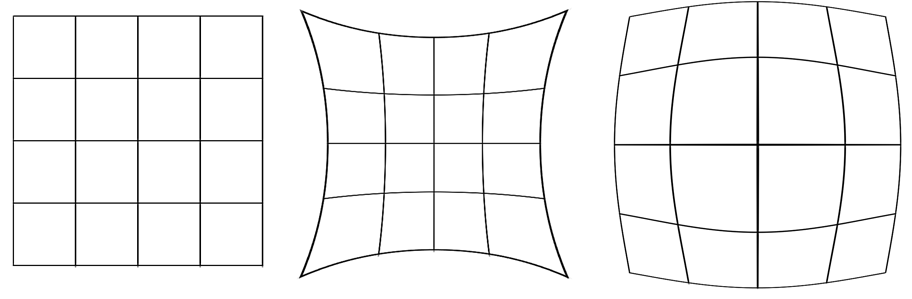
\includegraphics[width=0.5\textwidth]{img/camera/distortion.png}
	\caption{Examples of barrel and pincushion distortion on an image. Source: \cite{camera_models}}
	\label{fig:lense_distortion_types}
\end{figure}

For more information, see Hartley and Zisserman Multi View Geometry in Computer Vision~\cite{mvg_book}, Hata and Savarese course notes\cite{camera_models} and \acf{opencv} official documentation\cite{opencv_doc}. 

\subsection{Camera Intrinsic Calibration}
Calibrating a camera is the process on which the parameters of the model that describes its behavior are determined. For the pinhole camera model, this means determining the parameters of its intrinsic matrix, $K$, but also the distortion coefficients of the lens used~\cite{mvg_book, camera_models}. This parameters are called the intrinsic parameters and are independent of the scenario being viewed, if the focal length is keep constant. On the other hand, extrinsic camera parameters are different for every situation and scenario dependent.

The joint rotational-translation matrix, for a fixed camera in relation to the world frame of reference, is used to describe the rigid motion of an object on its front~\cite{opencv_doc}. Using this notion, Zhang proposed a method for calibration a camera based on the movement of a planar pattern in front of it, without the necessity to know how the planar plan was freely moved~\cite{Zhengyou2000, mvg_book}. Zhang also a maximum-likelihood estimation to miminize the error, using a such as Levenberg-Marquardt optimization~\cite{Levenberg1943}. Other techniques includes Tsai's algorithm \cite{Roger1987, mvg_book}, a 2-stage technique for camera calibration first presented in 1987, does not determins the camera center. A \ac{dlt} algorithm can also be used to determine the camera calibration parameters~\cite{mvg_book}.

Previous technics required 3 dimensional object based calibration \citeneeded, with expensive experimental apparatus or no calibration object, computing the intrinsic parameters only by rotating the camera on a static environment~\citeneeded. Bouguet also provides a Camera Calibration toolbox for \ac{matlab}~\cite{Jean_Yves} and \ac{opencv} also provides calibration algorithms based on Bouguet and Zhang~\cite{opencv}.

The calibration algorithm proposed by Zhang finds the correspondences between 2D and 3D points (see equations~\ref{eq:camera_transform} and~\ref{eq:camera_transform_full}), by variating the planar calibration object. For every configuration, a match between the two 2D and 3D points allows the determination of the projective matrix, $P$. However, if several translations and rotations of the pattern are made, it is possible to determine the intrinsic camera matrix, $K$, that is independent from the scene, using minimization algorithms. 

The correspondences between the 2D and 3D representations of the pattern can be made by finding the corners or circles on planar patterns~\citeneeded. Chessboards are the most common patterns used, allowing corner detection for each cell. Since the dimensions of the cell and their arrangment is known previously, it is possible to compute the orientation of the chessboard and to match the 2D to the 3D points \cite{Zhengyou2000, opencv_doc, mvg_book}.

\begin{figure}[H]
	\centering
	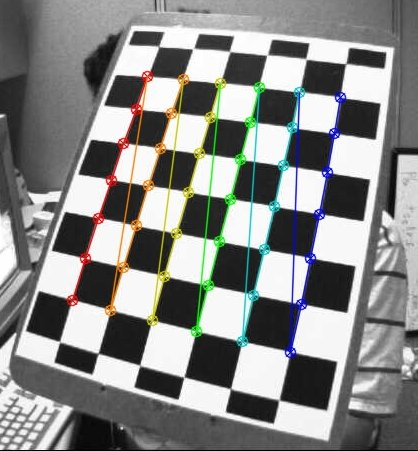
\includegraphics[width=0.4\textwidth, keepaspectratio]{img/camera/calib_pattern.jpg}
	\label{fig:opencv_calib_pattern}
	\caption{Chessboard calibration pattern with corners detection results show on image. Corner order is also given on the corner color. Source:~\cite{OpenCV_camera_calib}.}
\end{figure}

For error estimation, algorithm x\todo is used.

\subsection{Camera as a sensor for computer vision}
On the field of computer vision, several tools and libraries are available, capable of performing low image operations, image detection, filtering, among others. 

\begin{itemize}
	\item \textbf{BoofCV~\cite{boofcv}:} written in java, this library is oriented to real-time image operations, such as low-level image processing, camera calibration and feature/object  detection, tracking and recognition;
	\item \textbf{Dlib~\cite{dlib}:} modern C++ toolkit containing \acl{ml} algorithms and tools, some on the field of computer vision;
	\item \textbf{\ac{matlab} Computer Vision Toolbox\texttrademark~\cite{matlabcvtoolbox}:} toolbox for computer vision algorithms, 3D vision, and video processing systems. Can be perform object detection and tracking. Detects, extracts and matches features;
	\item \textbf{\acf{opencv}~\cite{opencv}:} open source library for C++, Python and C that implements \acl{sota} algorithms on computer vision;
	\item \textbf{Vlfeat~\cite{vlfeat}:} open source library for C that implements many \acl{sota} algorithms on computer vision;
	\item \textbf{SimpleCV~\cite{simplecv}:} Open source framework, written in python, that can be used to implement computer vision software using other libraries;
\end{itemize}

Since a goal of this research is to use Open-Source tools as far as possible (instead of using closed source tools or code that is harder to integrate with other libraries), \ac{matlab} \acl{cv} Toolbox\texttrademark~does not suit. The code of this research is mainly develop in C++ (see chapter \citeneeded), so Python and Java libraries will not be considered, resulting only in \ac{opencv} and Dlib (Vlfeat uses plain C, so also not ideal). 

\ac{opencv} has a great community and is considered by many research and industry as the \textit{de facto standard} library when refering to computer vision. Dlib is a robust library, but no significant differences can be when comparing with \ac{opencv}. Therefore, the final choice for a computer vision library is \ac{opencv}, due to the already implemented compatilibility with \ac{ros}.



%%%%%%%%%%%%%%%%%%%%%%%%%%%%%%%%%%%%%%%%%%% LIDAR %%%%%%%%%%%%%%%%%%%%%%%%%%%%%%%%%%%%%%%%%%

\section{Automotive \ac{lidar}}
\ac{lidar} sensors map their surroundings thanks to their capability of precisely measuring depth. Already used in topography, spectography and air poluttion studies, \ac{lidar} found its importance on the automotive industry as one of the sensors of autonomous cars and \ac{adas}\cite{Sullivan2016}. 

These maps produced by the \ac{lidar}, commonly represented as point clouds or mesh clouds models, (see figure~\ref{fig:bunny}), are one of the preferred method for \ac{slam} algorithms, which allow a vehicle without previous knowledge of its surroundings to autonomously navigate them - a crucial task for \ac{adas} on self-driving vehicles.

\begin{figure}[H]
	\centering
	\begin{subfigure}[c]{0.45\textwidth}
	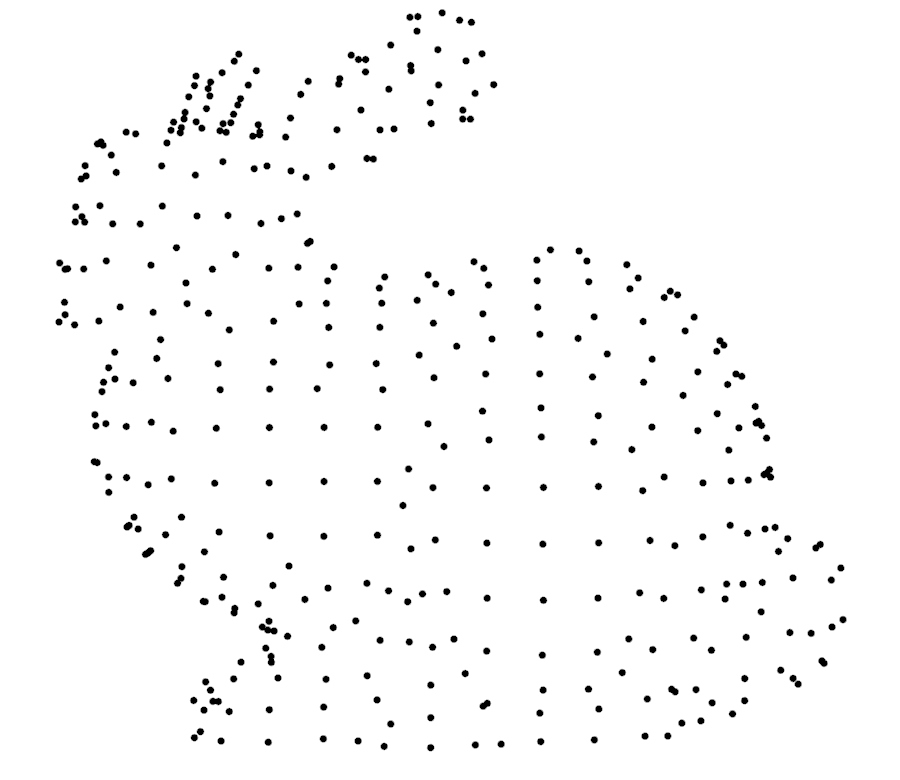
\includegraphics[width=\textwidth]{img/lidar/bunny_point.png}
		\caption{Point Cloud representation}
		\label{fig:bunnyPointCloud}
	\end{subfigure}
	\quad
	\begin{subfigure}[c]{0.4\textwidth}
		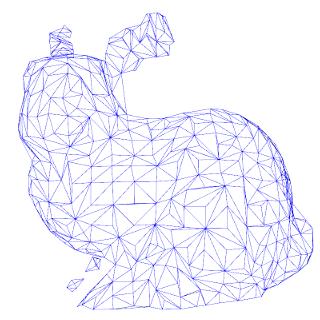
\includegraphics[width=\textwidth]{img/lidar/bunny_mesh.png}
		\caption{Mesh Cloud representation}
		\label{fig:bunnyMeshCloud}
	\end{subfigure}
	\caption{Standford bunny~\cite{bunny} point cloud (\subref{fig:bunnyPointCloud}) and mesh cloud (\subref{fig:bunnyMeshCloud})}
	\label{fig:bunny}
\end{figure}


Typically, four major technologies are used on the construction of a \ac{lidar}:

\begin{enumerate}
	\item \textbf{\ac{tof}:} the most common type, acquires depth information by measuring the time elapsed between the emission and reception of a \ac{laser} pulse reflected from a surrounding target \cite{Sullivan2016};
	\item \textbf{Flash:} organized in a matricial structure, similar to a camera \ac{ccd}, every element of the matrix contains a photodetector. A ``flash'' simultaneous illuminates all the \ac{fov}, and the reflected light intensity and time of arrival is measured to provide depth calculations; 
	\item \textbf{Phased Arrays:} using a microscopic array of antennas, similar to a \ac{radar}, the phase of each antenna is controled to allow the \ac{lidar} to sweep and/or focus on a specific area, using beamforming theory;
	\item \textbf{\ac{mems}:} operate by controlling the angle at which a rotating microscopic mirror is aligned with the \ac{laser}. By varying the angle a single line can be scanned and using multiple \acp{laser} with the samer mirror allows to scan vertically.

\end{enumerate}


\subsection{\acl{tof} vs Solid State \acp{lidar}}
Despite the existance of several technologies that can be used for \ac{lidar} construction, two majuor types of \ac{lidar} can be distringuished: \ac{tof} or Solid State. The former as no moving parts while the latter working principle is the rotational device.

To construct a \ac{tof} \ac{lidar}, a single pair of \ac{laser} and photodetector is assembled on a fast rotational device (typically 5 to 20 Hz), allowing that pair to measure a single line while rotating, creating a 2D \ac{lidar}. If multiple pairs are assembled together, with different polar angles, on a rotational device, the \ac{lidar} is said to be a 3D \ac{lidar}, since a total revolution can produce a three dimensional map of its surroundings~\cite{Sullivan2016}.

Solid State \ac{lidar} has no moving parts, and can either use flash or phased arrays on its construction, depending if it uses a flash of light to illumianate the scene or performs beam steering to scan the same scene. They are theoretically more reliable, durable cheaper and consume less power. However, this technology is not yet mature, which makes the current models impratical f or automotive. 

While \ac{tof} \acp{lidar} consumes more power, they can also achieve ranges until 100 meters \cite{vlp16, Sullivan2016} or even 300 meters\citeneeded, higher than solid state \ac{lidar}, which in best conditions reaches 50 meters~\citeneeded. That is due to the attenuation of the flash intensity, due to its power being inversely proportional with the distance squared\citeneeded. Considering the current \ac{sota} on \ac{tof} \ac{lidar} has less error (a few centimeters) than the \ac{sota} of Solid State \ac{lidar}.

However, Solid State \ac{lidar} have more point density than a \ac{tof} counterpart and measure the depth image of a scene on the same frame, theoretically allowing for more accurate data and faster refresh rates\citeneeded. 



%Combining the reliability of the depth measurement with the assemblage of multiple pairs of \ac{laser} and photodetectors on a fast rotational device (typically 5 to 20 Hz) creates one of the most appealing and reliable sensors for self-driving vehicles and \ac{adas}.

%Despite the relevance of the topic for the massification of self-driving vehicles and the hazardous impact on \Gls{adas} reliability, the research topic presented in this paper has received very reduced attention by the research community. 
%A major \ac{lidar} manufacture also addresses the problem of mutual interference of the \ac{lidar} sensors on the same vehicle, by allowing their synchronization and \ac{laser} firing in different instants \cite{vlp16}.

\section{Object Detection}
Several paid and cloud based alternatives exist, such as Amazon Rekognition~\ref{awsRecognition}, Google Could Vision \ac{api}~\cite{googlevision}, IBM Watson Visual Recognition~\cite{watson} and Microsoft Computer Vision software~\cite{azurecv}. 




\section{\ac{lidar} Interference}
\ac{tof} \ac{lidar}s basic principle implies that when a \ac{laser} pulse is emitted, three different scenarios are possible, being the first one the only one that produces a valid measurement:

\begin{enumerate}
\item The \ac{laser} pulse returns, due to the reflection of an obstacle;
\item The \ac{laser} pulse does not return;
\item The \ac{laser} pulse returns with intensity below the noise floor.
\end{enumerate}

Interference and crosstalk between the pairs of \acp{laser} and photodetectors on a \ac{lidar} are mitigated with different firing offsets, or in the case of mutual interference between \ac{lidar}, it is possible to synchronize their firing time using specialized clock signals \cite{vlp16}.

However, in a society when self-driving vehicles coexist, another scenario is possible: a \ac{lidar} `A'' fires a \ac{laser} pulse that is received, directly or indirectly, by the photodetector on a \ac{lidar} `B''. Since \ac{lidar} `B'' measures the distance to an obstacle by measuring the time between the firing and reception of its own \ac{laser} pulse, the reception of another \ac{laser} pulse results in an erroneous measure with an unpredictable behavior. If this interference is significant, the reliability of the \ac{lidar}, and consequently autonomous vehicles and \ac{adas}, is seriously undermined due to the incapability to accurately mapping their surroundings.

To the best of the author's knowledge, despite the relevance of the topic to a society of self-driving cars, there are only available the studies conducted by Kim \etal \cite{Kim2017, Kim2015}, which seek to characterize this interference; and by Retterath and Laumeyer \cite{Al.2013}, seeking to provide an apparatus for reducing the mutual interference of \ac{lidar} sensors on the same vehicle.


Kim \etal research %despite using a 2D \ac{lidar}%instead of a 3D \ac{lidar}
is the only study to use two independent 2D \ac{lidar}s interfering with each other. Kim \etal results indicate that interference has spatial and temporal locality \cite{Kim2015} and in any given time, in Kim's setup, a data point has 0.05 \% probability of being interfered \cite{Kim2015}.
The former states that if a particular angle is interfered, the following angles are likely to also be interfered; while the latter indicates that if a measure is interfered, on the following frame that same measure is also likely to be interfered. 
%However, 


